\ifpdf
    \graphicspath{{Chapter3/Figs/Vector/}{Chapter3/Figs/PDF/}{Chapter3/Figs/}}
\else
    \graphicspath{{Chapter3/Figs/Raster/}{Chapter3/Figs/}}
\fi


\chapter{Linear Time Gaussian Processes on HyperSpheres}
\label{chapter:vish}

Stationary kernels, i.e. translation invariant covariances, are ubiquitous in machine learning when the input space is Euclidean. When working on the hypersphere, their spherical counterpart are dot-product kernels, which are invariant to rotations. They are the main object under study in this chapter. In \cref{sec:rkhs-dotproduct-kernels}, we first show how we can construct the Reproducing Kernel Hilbert Space (RKHS) of dot-product kernel on the hypersphere. \Cref{sec:vish} uses the RKHS to construct an efficient variational interdomain inducing variable for Gaussian processes on the hypersphere. We will then show how to expand the GP onto the complete domain $\Reals^d$ and conclude with a series of experiments, showing the speed and accuracy of the proposed approach.

\section{Mercer Representation of Dot-Product Kernels}
\label{sec:rkhs-dotproduct-kernels}

Consider the unit sphere in $\Reals^d$  as the input domain
\begin{equation}
    \mathcal{X} = \dsphere = \{x \in \Reals^d: \norm{x}_2 = 1\}
\end{equation}
and $\nu$ to be the Lebesgue measure on $\dsphere$, so that
\begin{equation}
    \darea = \int_{\dsphere} \calcd{\nu(x)} = \frac{2 \pi ^ {d/2}}{\Gamma(d/2)}.
\end{equation}
is the surface area of $\dsphere$. We adopt the usual $L_2$ inner product for functions $f: \dsphere \rightarrow \Reals$ and $g: \dsphere \rightarrow \Reals$ restricted to the sphere 
\begin{equation}
     \langle f, g\rangle_{L_{2}(\dsphere)} = \frac{1}{\darea} \int_{\dsphere} f(x)\,g(x) \, \calcd{\nu(x)}.
\end{equation}

We define a dot-product kernel, also known as a zonal kernel (we will use both terms interchangably), as a p.d. kernel of the form
\begin{equation}
    k(x, x') = \kappa(x\transpose x'),
\end{equation}
where $\kappa: [-1, 1] \rightarrow \Reals$ is a continuous function and referred to as the shape function. In other words, dot-product kernels only depend on the distance on the great circle between two inputs, rather than their location. They are the counterpart of stationary kernels $k(x, x') = \kappa(x - x')$, who are functions of the difference only. For example, where stationary kernels are translation invariant, dot-product kernel are rotationally invariant.

% TODO: example Arc Cosine and Stationary kernels on the hypersphere


We can associate a kernel operator $\mathcal{K}$ to a zonal kernel, as explained in \cref{section:theory:spectral-formulation}, which exhibits the form
\begin{equation}
    \label{eq:kernel-operator-zonal}
  \mathcal{K} f = \int_{\dsphere} \kappa(x\transpose\cdot) f(x) \calcd{\nu(x)}.
\end{equation}
To construct a Mercer representation of a zonal kernel's RKHS we require the eigensystem of the kernel operator $\mathcal{K}$, or, equivalently, the set of eigenfunctions $\{\phi_n\}$ and associated eigenvalues $\{\lambda_n\}$ for which
\begin{equation}
    \mathcal{K} \phi_n = \lambda_n \phi_n\qquad\text{and}\qquad \langle \phi_n, \phi_m \rangle_{L_2(\dsphere)} = \delta_{nm}.
\end{equation}

To obtain the eigensystem of $\mathcal{K}$, we will show that $\mathcal{K}$ commutes with the Laplace-Beltrami operator $\LaplaceBeltrami$, henceforth referred to as simply the Laplacian or the Laplace operator. We want to remind the reader that commuting operators share the same eigenfunctions, but not necessarily the same eigenvalues. Therefore, to find the eigenfunctions of the kernel operator $\mathcal{K}$, it suffice to find the eigenfunctions of the Laplacian. Fortunately, the diagonalisation of the Laplace operator on $\dsphere$ is a well-studied problem. In the following paragraph we first proof the commutativity of the operators before covering the definition of the RKHS.

\paragraph{Commutativity of $\mathcal{K}$ and $\LaplaceBeltrami$.}
We now proof that the Laplacian and the kernel operator of zonal kernels commute. For this, we first show that for zonal kernels and $x,s \in \dsphere$ the following property holds
\begin{align}
    \LaplaceBeltrami_x k(x, x') 
     &= \nabla_x \cdot \nabla_x \kappa(x\transpose x') && \text{Definition $\LaplaceBeltrami$ and zonal kernels}\\
     &= \nabla_x \cdot (x' \kappa'(x\transpose x'))  && \text{Chainrule} \\
     &= \norm{x'}^2 \kappa''(x\transpose x') = \kappa''(x \transpose x') && \text{Because } \norm{x'} = 1.
\end{align}
Similarly, for $\LaplaceBeltrami_s k(x, x')$ we obtain $k''(x \transpose x')$, and as a result
\begin{equation}
    \label{eq:LaplaceBeltrami-x-s}
\LaplaceBeltrami_x k(x, x') = \LaplaceBeltrami_{x'} k(x, x').
\end{equation}
Relying on integration by parts and the previous result, we obtain
\begin{align}
    \mathcal{K} \left[\LaplaceBeltrami f\right] &= \int_{\dsphere} k(x, x') \left[\LaplaceBeltrami_x f(x)\right] \calcd{\nu(x)} && \text{Definition $\mathcal{K}$, \cref{eq:kernel-operator-zonal}}\\
    &= \int_{\dsphere} f(x) \LaplaceBeltrami_x k(x, x')  \calcd{\nu(x)} && 2\,\times\,\text{Integration by parts}\\
    &= \int_{\dsphere} f(x) \LaplaceBeltrami_{x'} k(x, x')  \calcd{\nu(x)}  && \text{\cref{eq:LaplaceBeltrami-x-s}} \\
    &= \LaplaceBeltrami \left[ \mathcal{K} f \right]
\end{align}
which shows that the two operators commute and in turn implies that they share the same eigenfunctions. This result is of particular relevance to us since there is a huge body of literature on diagonalisation of the Laplace-Beltrami operator on $\dsphere$, and that it is well known that its eigenfunctions are given by the spherical harmonics. The spherical harmonics $\phi_{n,j}$ form an orthonormal basis for the square-integrable functions on the hypersphere. They are indexed with a level $n$ and an index within each level $j \in \{1, \dots, \dnumharmonicsforlevel\}$. See \cref{appendix:spherical-harmonics} for a comprehensive introduction to spherical harmonics, as well as a practical algorithm to compute them for relatively large $d$. \Cref{fig:harmonics} shows the first 4 levels of spherical harmonics in $\Reals^3$.

The above reasoning about the commutativity of the Laplace-Beltrami and kernel operator and the diagonalisation of the Laplace-Beltrami operator by the spherical harmonics, can be summarised by the following theorem:
\begin{theorem}[Mercer decomposition]
Any zonal kernel $k(x, x') = \kappa(x\transpose x')$ on the hypersphere can be decomposed as
\begin{equation}
\label{eq:kernel-form}
    k(x, x') = \sum_{n=0}^{\infty} \sum_{j=1}^{\dnumharmonicsforlevel} \lambda_{n} \phi_{n,j}(x) \phi_{n,j}(x'),
\end{equation}
where $x,x' \in \dsphere$ and $\lambda_{n}$ are positive coefficients, $\phi_{n,j}$ denote the elements of the spherical harmonic basis in $\dsphere$, and $\dnumharmonicsforlevel$ corresponds to the number of spherical harmonics for a given level $n$. As a result of the Funk-Hecke theorem, the associated eigenvalues only depending on the level $n$
\begin{equation}
    \label{eq:compute-eigenvalues}
        \lambda_{n} = \frac{\omega_{d}}{C_n^{(\alpha)}(1)} \int_{-1}^1 \kappa(t)\,C_n^{(\alpha)}(t)\,(1 - t^2)^{\frac{d-3}{2}} \calcd{t},
\end{equation} 
where $C_n^{(\alpha)}$ is the Gegenbauer polynomial of degree $n$, $\alpha = \frac{d-2}{2}$, $\omega_d$ is a constant that depends on the surface area of the hypersphere. Analytic expressions are given in \cref{appendix:spherical-harmonics}.
\end{theorem}
Although it is typically stated without a proof, this theorem is already known in some communities (see \citet{wendland2005} for a functional analysis exposition, or \citet{peacock1999cosmological} for its use in cosmology). Given the Mercer decomposition, we can equivalently, define the associated RKHS as
\begin{equation}
    \label{eq:rkhs-sphere}
    \rkhs = \left\{
    f = 
    \sum_{n=0}^\infty \sum_{j=1}^{\dnumharmonicsforlevel} {f}_{n,j} \sh_{n, j}:
    \norm{f}_{\rkhs} < \infty
    \right\},
    \quad\text{where}\quad
    \langle g, h \rangle_{\rkhs} = 
    \sum_{n,j}
            \frac{{g}_{n, j} {h}_{n, j}}{\lambda_{n}}
\end{equation}
is the \emph{reproducing} inner product between two functions $g,h \in \rkhs$. The reproducing property of the RKHS implies that for $f \in \rkhs$: $f(x) = \langle f, k(x, \cdot) \rangle_\rkhs$, which will enable the constuction of spherical harmonic inducing features of discussing in the following section.

%%%%%%%%%%%%%%%%%%%%%%
\section{Variational Spherical Harmonic Gaussian Processes}
\label{sec:vish}

We can now build on the results from the previous section, combined with interdomain inducing variables (see \cref{section:interdomain-inducing-variables}), to propose a novel sparse variational GP model. Specifically, we are using interdomain inducing variables that are defined through the zonal kernel's RKHS inner product. As a result we will obtain expressive features $\kux$ that exhibit non-local influence, and efficient inducing variables that induce diagonal structure in $\Kuu$. We achieve this by defining the inducing variables $u_m$ to be the inner product between the GP and spherical harmonics:\footnote{Note that in the context of inducing variables, we switch to a single integer $m$ to index the spherical harmonics and order them first by increasing level $n$, and then by increasing $j$ within a level.}
\begin{equation}
  u_m = \langle f, \sh_m\rangle_{\rkhs}\quad\text{for}\quad m \in \{1, \ldots, M\}.
\end{equation}
To leverage these new inducing variables we need to compute two quantities: 1) the covariance between $u_m$ and $f$ for $\kux$, and 2) the covariance between the inducing variables themselves for the $\Kuu$ matrix. Firstly, we compute the covariance of the inducing variables and the GP
\begin{align}
   \left[\kux \right]_m 
    &= \ExpSymb[f(\cdot)\,u_m] && \text{Definition covariance} \\
    &= \ExpSymb[f(\cdot)\,\langle f, \sh_m\rangle_{\rkhs}] && \text{Definition $u_m$} \\
    &= \langle k(\cdot, \cdot), \sh_m \rangle_{\rkhs}   && {k(\cdot, \cdot) = \ExpSymb[f(\cdot) f]} \\
    &= \phi_{m}(\cdot) && \text{Reproducing property.}
\end{align}
where we relied on the linearity of the expectation and the inner product and the reproducing property of $\rkhs$. Interestingly, using this construction we obtain the RKHS basis functions $\{\phi_m\}$ as the features for the sparse approximation. Secondly, the covariance between the inducing variables is given by
\begin{equation}
    \left[\Kuu \right]_{m, m'} = \ExpSymb \left[u_m\,u_{m'} \right] 
    % = \ExpSymb \left[ \langle f, Y_{m} \rangle  \langle f, Y_{m'} \rangle  \right] 
    = \langle \sh_{m}, \sh_{m'} \rangle_{\rkhs} 
    = {\delta_{mm'} \over \lambda_m},
\end{equation}
where $\delta_{mm'}$ is the Kronecker delta. Crucially, this means that $\Kuu$ is a diagonal matrix $\textrm{diag}(\lambda_1, \lambda_2, \ldots, \lambda_M)^{-1}$ containing the inverse eigenvalues on its diagonal. Finally, substituting $\Kuu$ and $\kux$ into the sparse variational approximation (\cref{eq:qf}) leads to
\begin{equation}
\begin{aligned}
    q(f) =
    \GP\Big(\bm{\phi}^\top(x)\,\vm;\ k(x, x') + &{\bm{\phi}}^\top(x)(\MS - \Kuu){\bm{\phi}}(\vx') \Big),\\ &\text{with}\quad\bm{\phi}(x) = [\lambda_m \phi_m(x)]_{m=1}^M \in \Reals^M.
\end{aligned}
\end{equation}
Through this construction we created a SVGP model with 1) spherical harmonic basis functions, and 2) a diagonal $\Kuu$ matrix, which means that we do not incur the cubic cost of matrix inversion in the evaluation of the model or the variational lower bound. The sperical harmonic basis functions have as advantage that they have global support, so that even a few of them are able to capture the rough shape of the function. This is similar to the Fourier series approximation, in which the first few terms are already able to roughly approximate the function. In the experiments we will discuss this phenomenon in more detail.

Note that while the inducing variables $\{u_m\}$ are independent under the prior (i.e. $p(\vu) = \NormDist{\bm{0}, \Kuu}$ with $\Kuu$ a diagonal matrix), that does not imply that the posterior over the inducing variables is diagonal as well. As a result, we still parameterise $q(\vu) = \NormDist{\vm, \MS}$, where $\MS$ is a full-rank matrix which captures all the pairwise covariances.

\section{Homogeneous Extension to $\Reals^d$}

\begin{figure}[t]
\centering
\begin{minipage}{.48\textwidth}
  \centering
  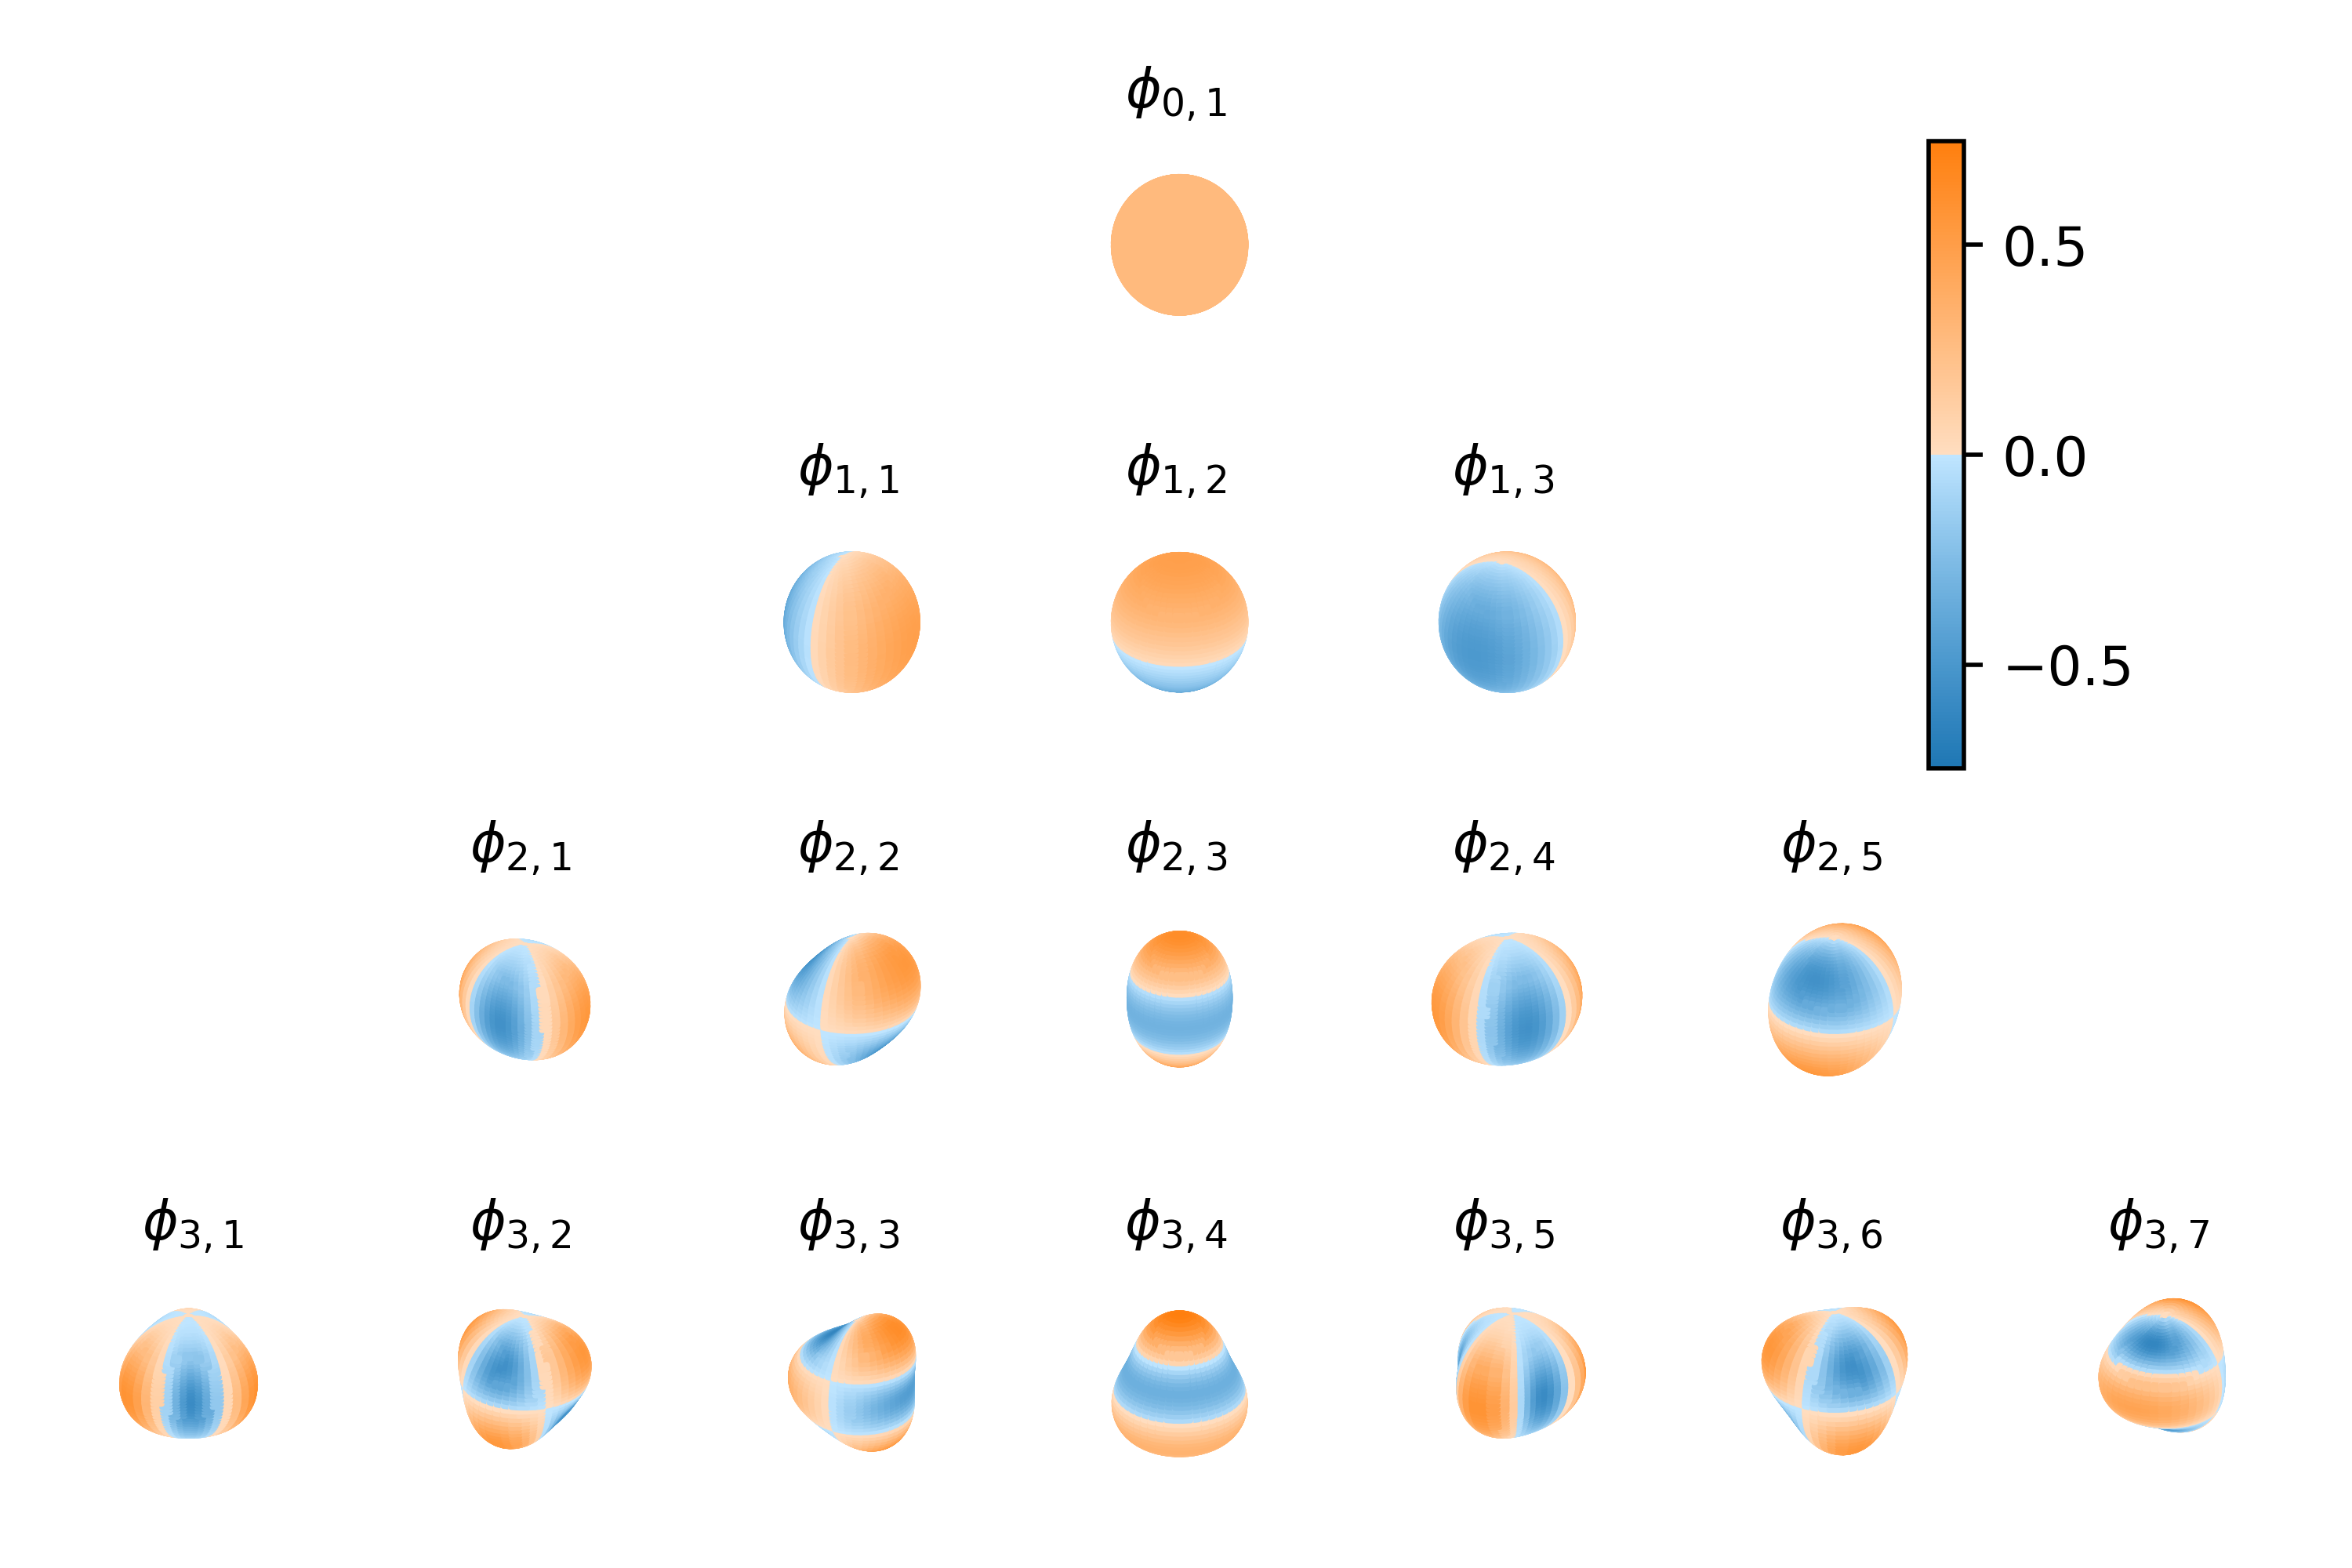
\includegraphics[width=\linewidth]{harmonics}
  \captionof{figure}{Spherical Harmonics on $\sphere^2$}
  \label{fig:harmonics}
\end{minipage}\hfill
\begin{minipage}{.48\textwidth}
  \centering
  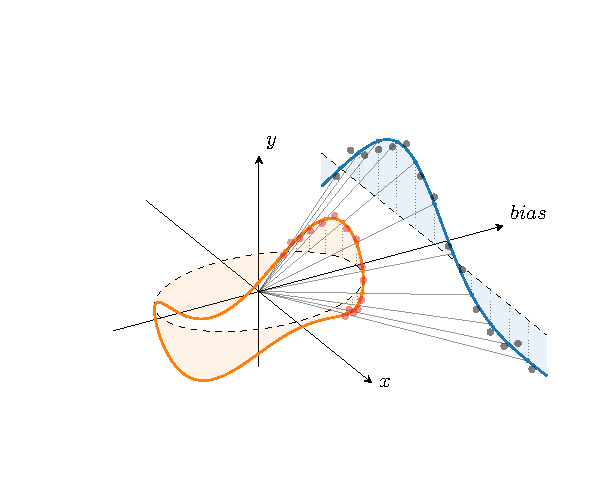
\includegraphics[width=\linewidth,trim=1.5cm 1.6cm 1.cm 1.55cm,clip=true]{mapping}
  \captionof{figure}{Example Homogeneous Extension}
  \label{fig:mapping}
\end{minipage}
\end{figure}

So far, the domain of interest has been the hypersphere $\dsphere$ . However, most regression problems in machine learning have inputs defined on the complete Euclidean space. We can address this problem as follows. Consider $x \in \Reals^{d-1}$ to be the input of the dataset and $y \in \Reals$ the corresponding output.
\begin{enumerate}
    \item We start by concatenating the datapoint $x \in \Reals^{d-1}$ with a bias term $b \in \Reals$ to obtain $x = [x, b] \in \Reals^d$. This operation corresponds to embedding the $(d\!-\!1)$-dimensional datapoint on a plane in $\Reals^d$ where $x_d = b$.
    \item Subsequently, the data is linearily projected to the hypersphere through normalisation: $x = {x \over \norm{x}} \in \dsphere$ and $y = {y \over \norm{x}}$.
    \item Based on the projected data we learn $f \sim \GP$ on $\dsphere$ using the approach outlined in the previous section.
    \item Finally, the function on the sphere can be extended to the whole domain by a homogeneous extension thereof: $g: \Reals^d \rightarrow \Reals$ with $g(x) = \norm{x} f({x \over \norm{x}})$. In other words, by linearily extrapolating the values on the hypersphere we obtain the values of the function in the data plane.
\end{enumerate}
This procedure is explained in \cref{fig:mapping}, which gives an illustration of the mapping between a 2D dataset (grey dots) embedded into a 3D space and its projection (orange dots) onto the unit half-circle using a linear mapping.

Although this setup may seem very arbitrary, it is inspired by the important works on the limits of neural networks as Gaussian processes. The first order Arc Cosine kernel \citep{cho2009kernel} is one of the most well-known examples, and mimics the computation of infinitely wide fully connected layers with ReLU activations. Let $\sigma(t) = \max(0, t)$, then the covariance between function values of $f(x) = \sigma(w\transpose x)$ for $w \sim \NormDist{0, d^{-1/2} \Eye_d}$ and $w \in \Reals^d$ is given by
\begin{equation}
\label{eq:arccosine}
    k(x, x') = \Exp{w}{\sigma(w\transpose x)\, \sigma(w\transpose x')} = \underbrace{\norm{x} \norm{x'}}_{\text{radial}}\ \underbrace{\frac{1}{\pi}\big( \sqrt{1 - t^2} + t\, (\pi - \arccos t) \big)}_{\text{angular (shape function) } \kappa(t)},
\end{equation}
where $t = \frac{\vx^\top \vx'}{\norm{\vx}\norm{\vx'}}$. Indeed, we observe how the first order Arc Cosine kernel factorises in a radial and an angular component. The radial component simply linearly extrapolates the values on the hypersphere, while the angular component encodes the covariance on the hypersphere and is only a function of the geodestic distance. This factorisation exactly matches our setup. We can generalise the zonal kernels of the previous section and their corresponding RKHS to the complete domain $\Reals^d$ using the following definition
\begin{equation}
    k(x, x') = \norm{x} \norm{x'} \kappa\left( \frac{x^\top x'}{\norm{x}\norm{x'}} \right), % \quad \text{and} \quad f(x) = \norm{x} f\left({x \over \norm{x}}\right).
\end{equation}
which leads to an RKHS consisting of functions defined on $\Reals^d$ of the form $g(x) = \norm{x}\,f(\frac{x}{\norm{x}})$, where $f \in \rkhs$ (from \cref{eq:rkhs-sphere}) is defined on the unit hypersphere but fully determines the function on $\Reals^d$.


\section{Related Work}

\begin{figure}[tbh!]
  \centering
\begin{subfigure}{0.49\textwidth}
  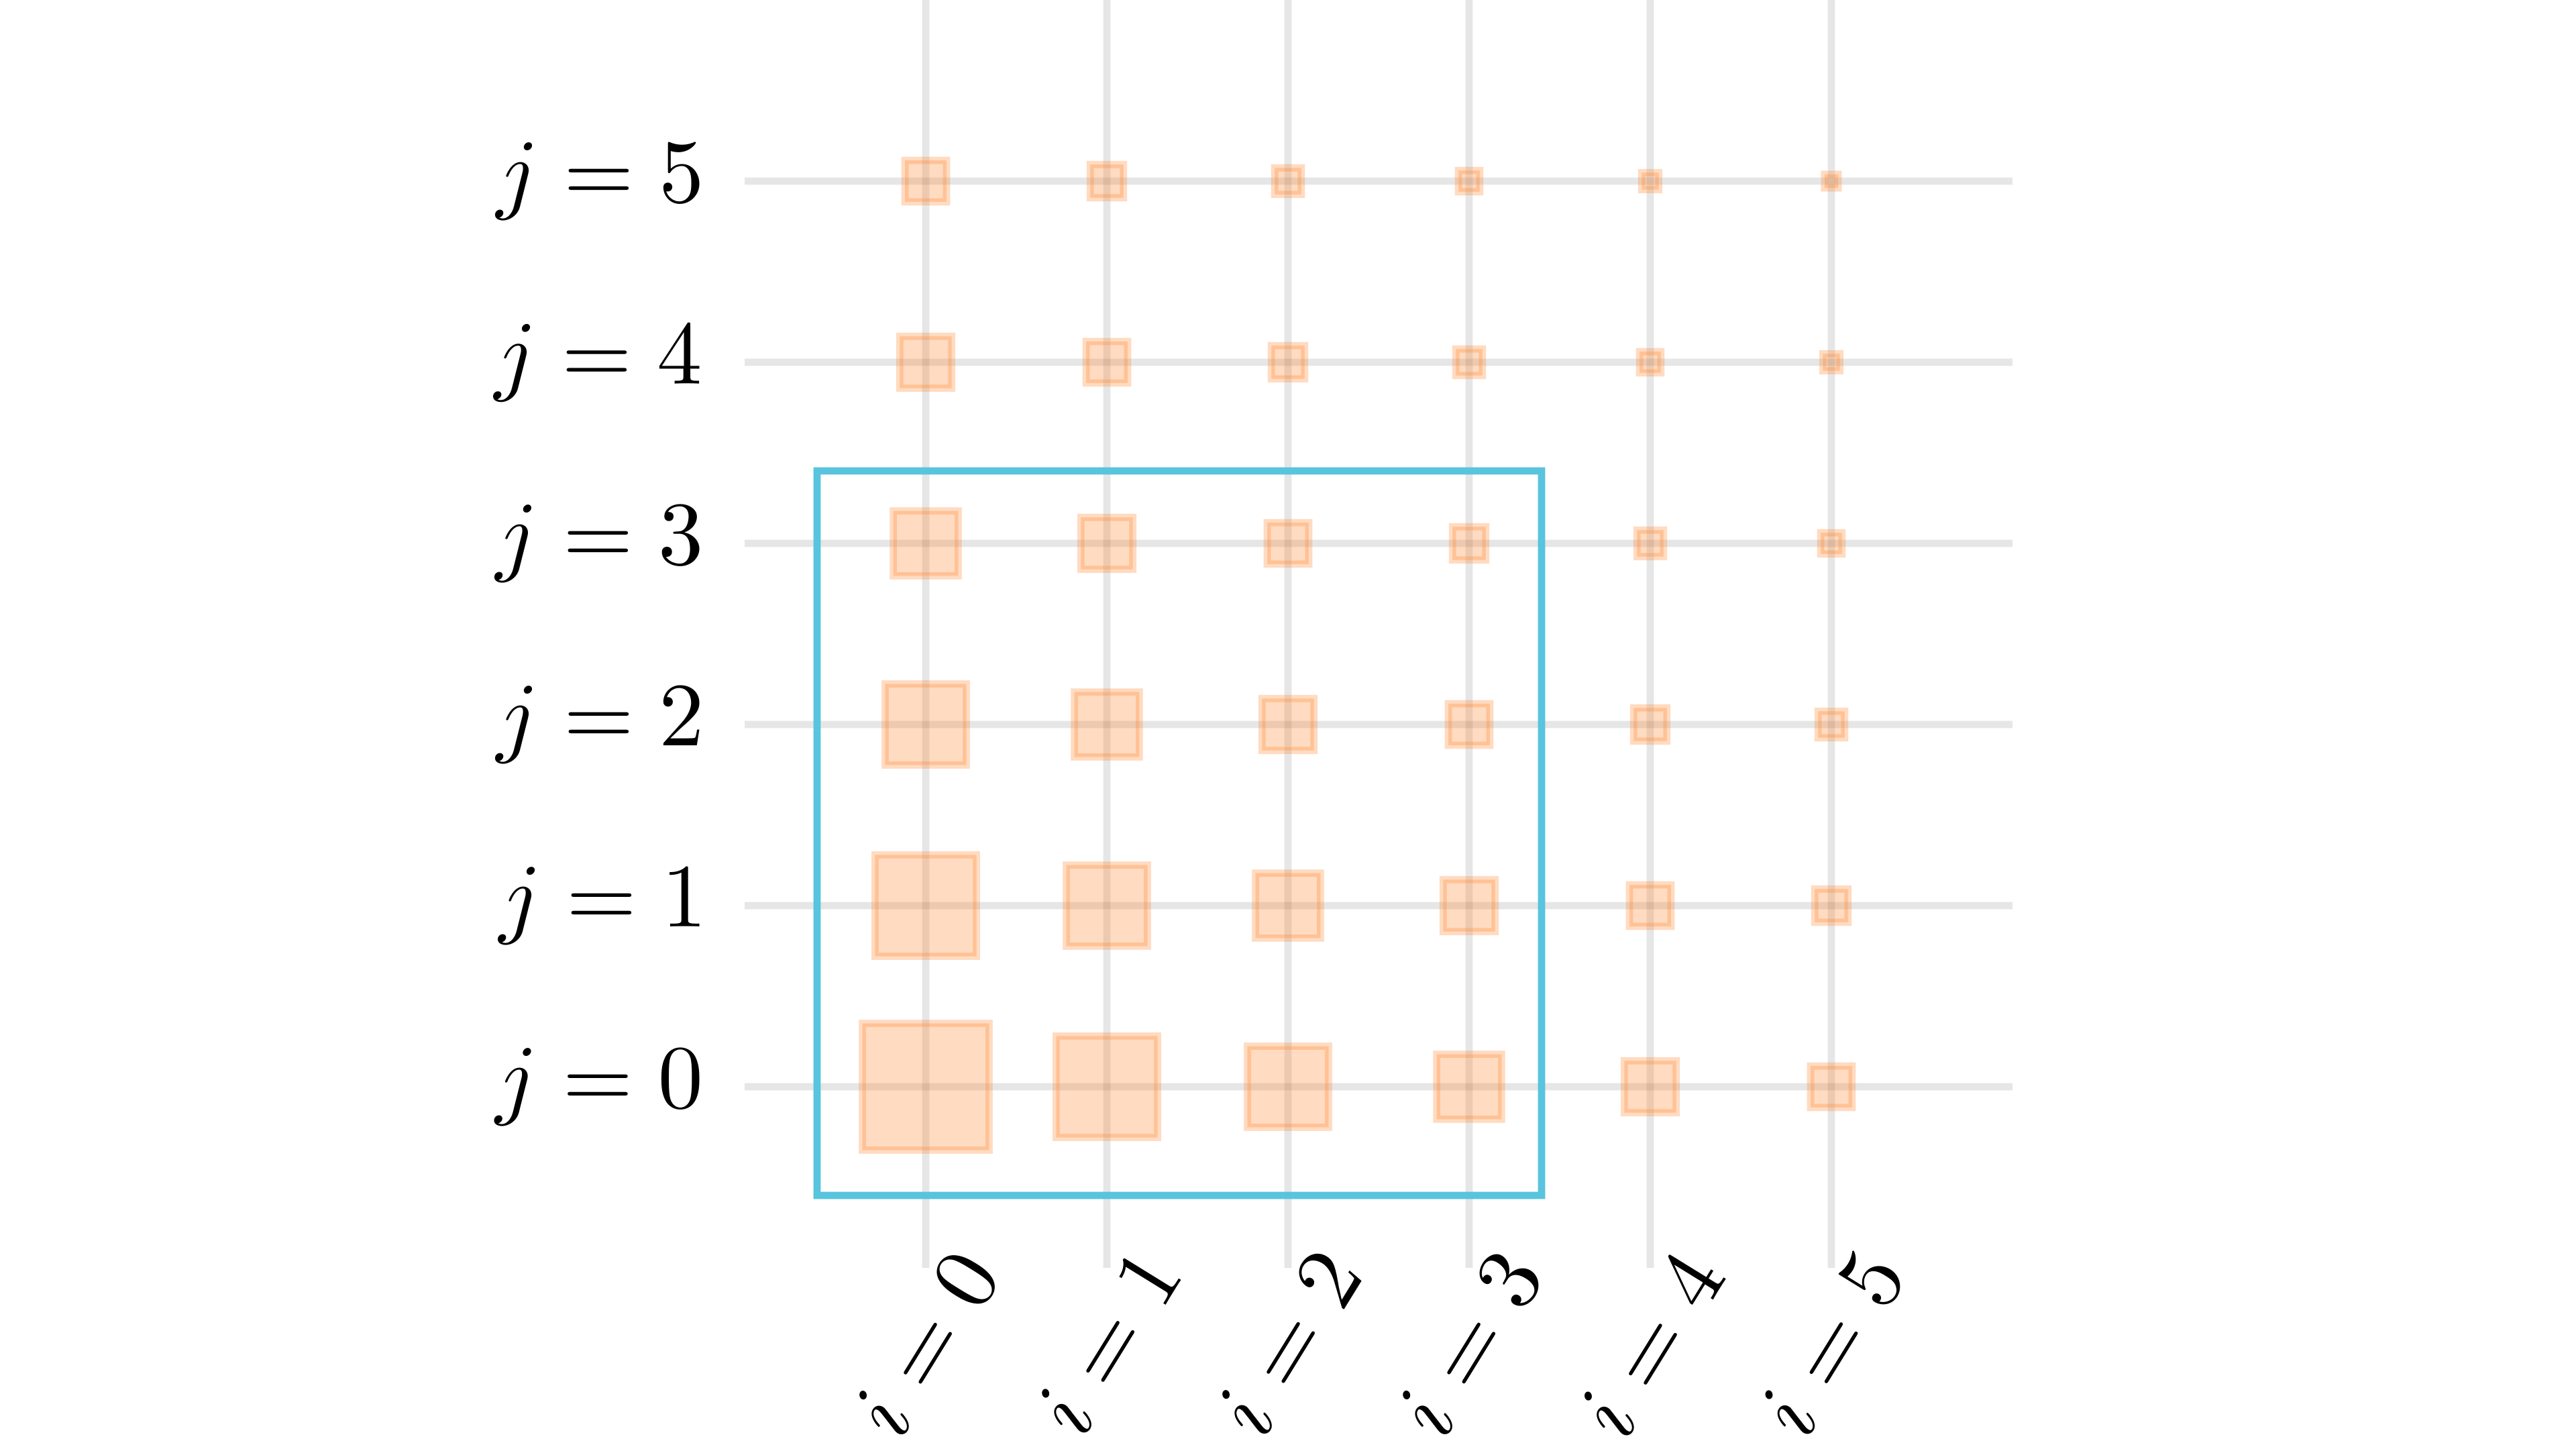
\includegraphics[width=\textwidth]{VFF}
  \caption{VFF}
  \label{fig:decay-vff}
\end{subfigure}\hfil % <-- added
\begin{subfigure}{0.49\textwidth}
  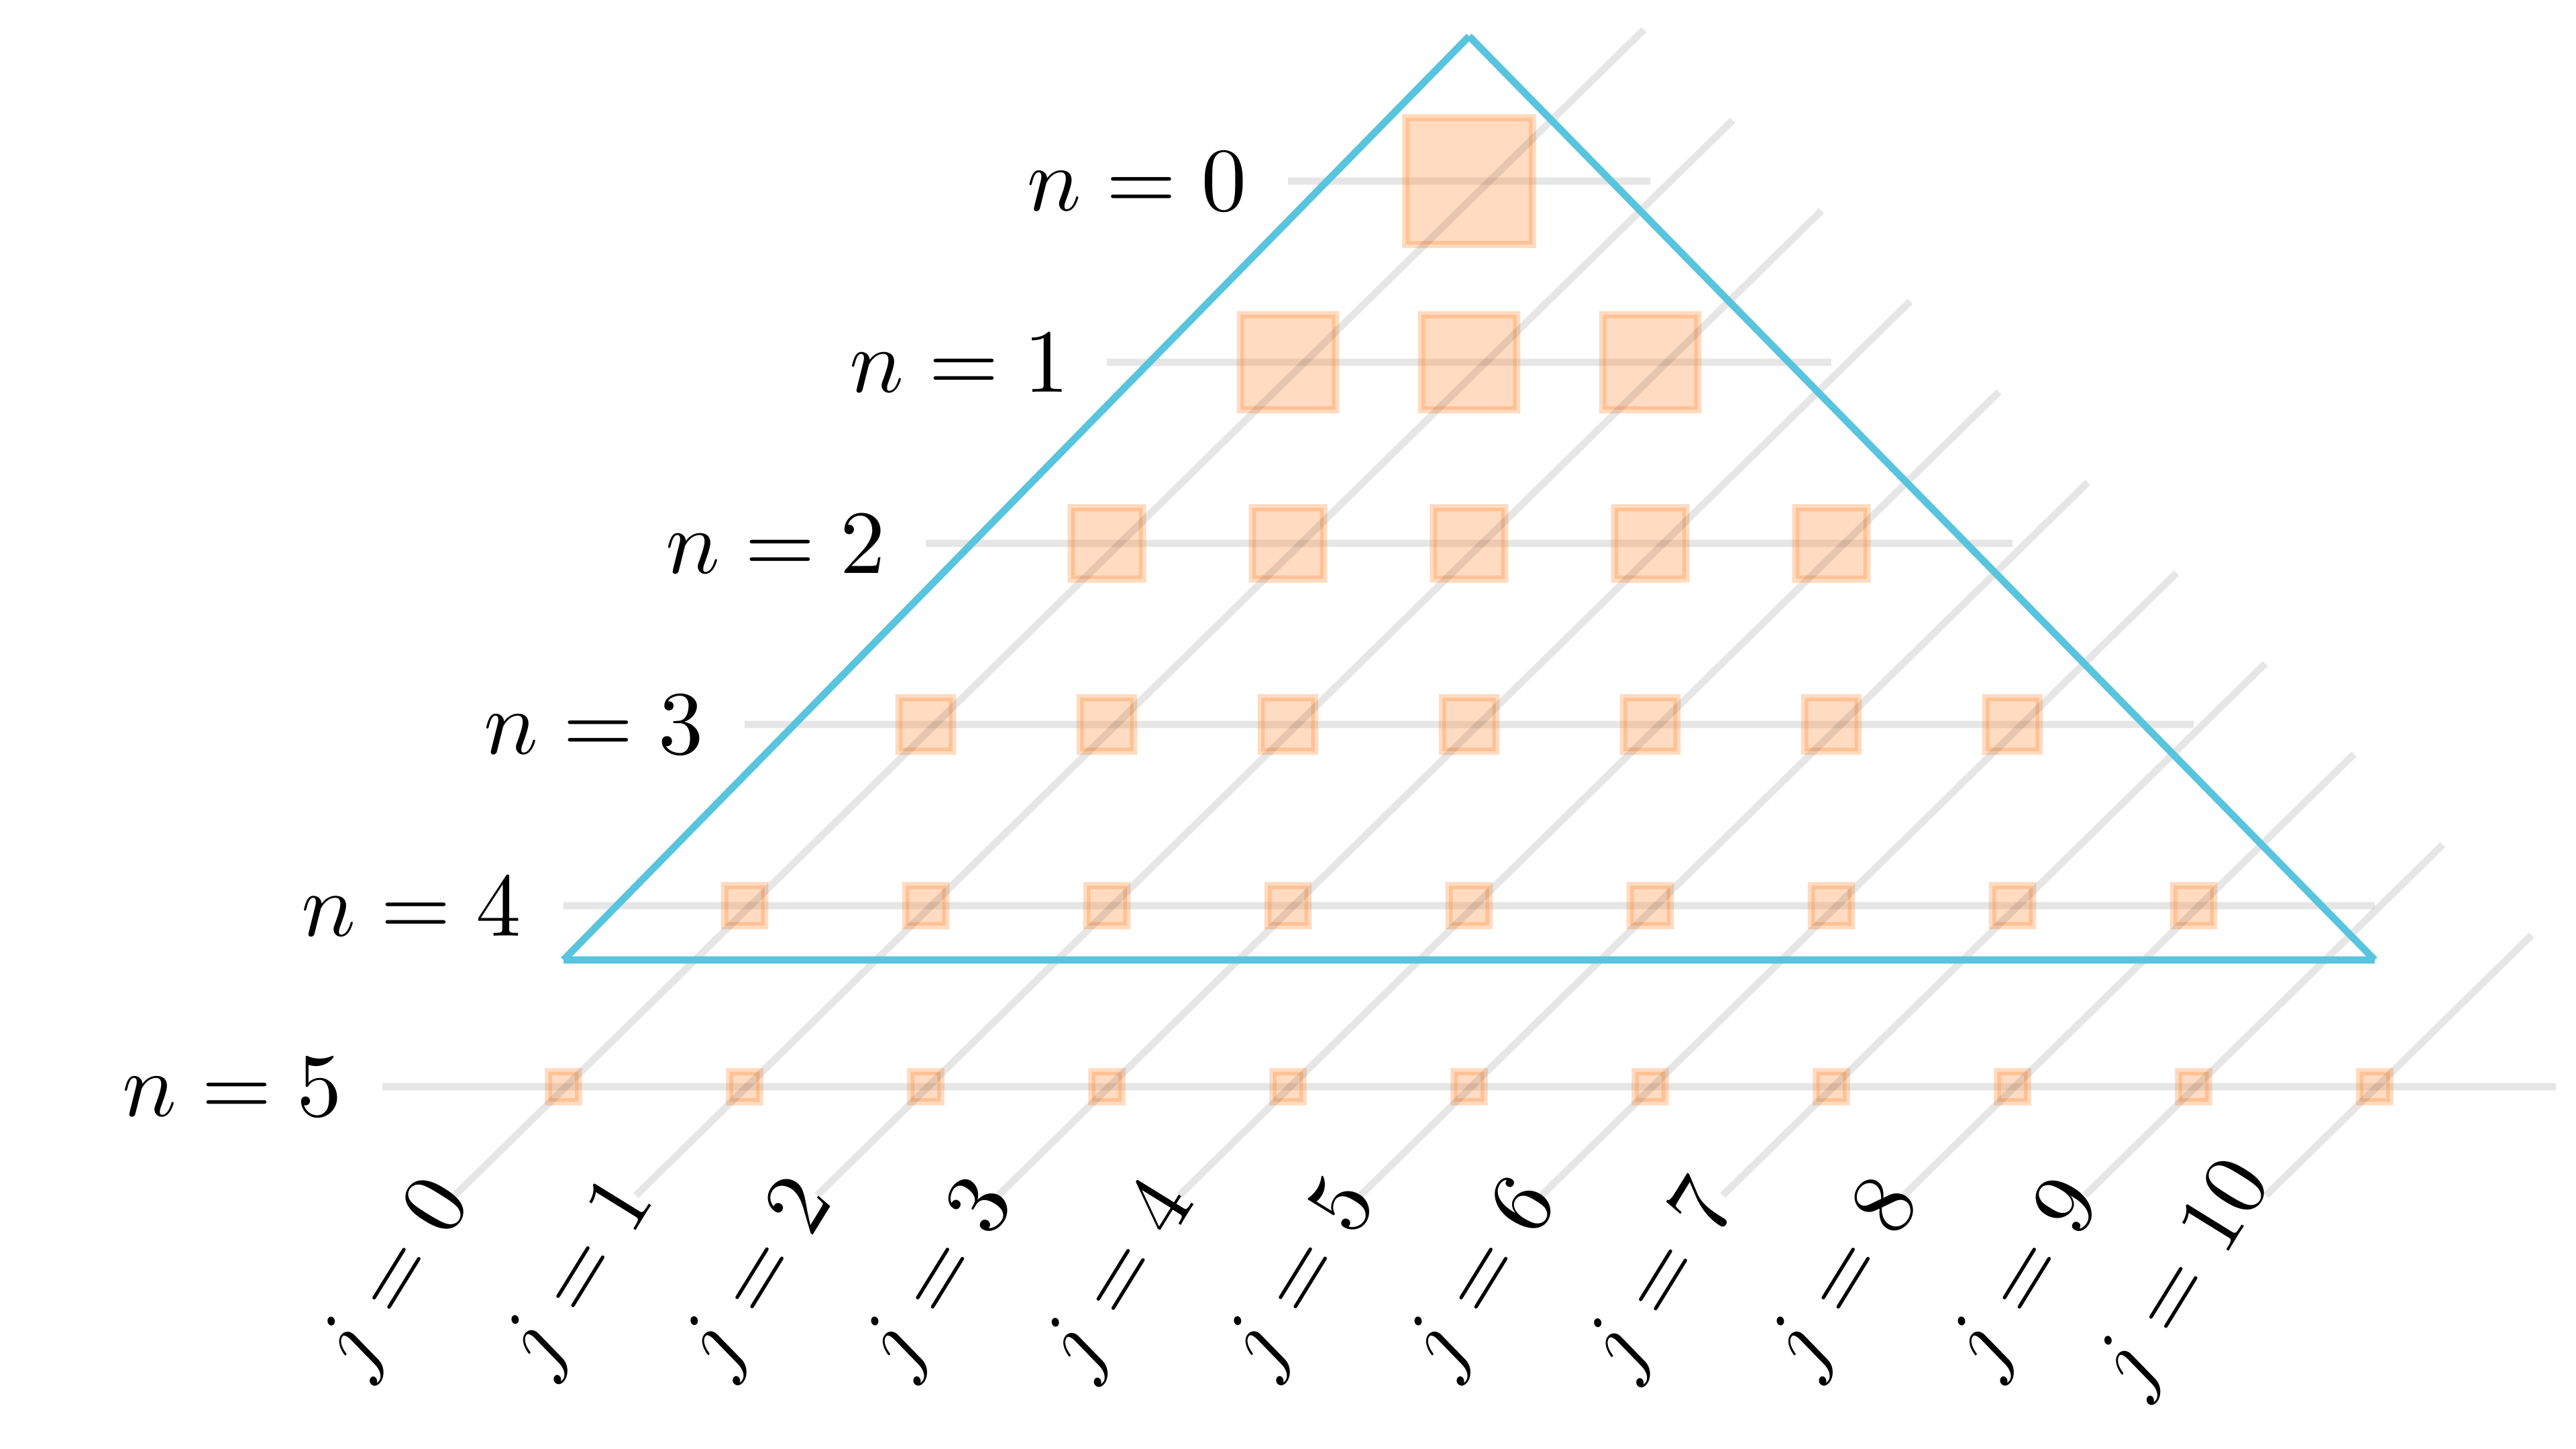
\includegraphics[width=\textwidth]{VISH}
  \caption{VISH}
  \label{fig:decay-vish}
\end{subfigure}\hfil % <-- added
\caption{Decay rate}
\label{fig:decay-vff-vs-vish}
\end{figure}

\begin{enumerate}
    \item Variational Fourier Features
    \item Variational Orthogonal Features
\end{enumerate}


% especially the \emph{arc-sine} kernel \citep{williams1998computation} and the \emph{arc-cosine} kernels \citep{cho2009kernel}. An arc-cosine kernel corresponds to the infinitely-wide limit of a single-layer ReLU-activated network with Gaussian weights. Let $\vx, \vx' \in \Reals^{d}$, such that $x_d = x'_d = b$, be an augmented input vector whose last entry corresponds to the bias. Then the arc-cosine kernel can be written as
% \begin{multline*}
%     k_{ac}(\vx, \vx') = \norm{\vx}\,\norm{\vx'}\,\underbrace{\frac{1}{\pi} \big( \sin \theta + (\pi - \theta) \cos \theta \big)}_{=J(\theta)}, \\
%     \text{where}\quad\theta = \cos^{-1}\left(\frac{\vx\transpose\vx'}{\norm{\vx}\norm{\vx'}}\right).
% \end{multline*}
% The kernel is a function of the norm of the inputs $\norm{\vx}\,\norm{\vx'}$ and a factor $J(\theta)$ that only depends on the geodestic distance $\theta$ (or the great-circle distance) between the projection of $\vx$ and $\vx'$ on the unit hypersphere. 


\section{Experiments}

We evaluate our method Variational Inference with Spherical Harmonics (VISH) on a regression and a classification problem to demonstrate that VISH performs competitively in terms of accuracy and uncertainty quantification, while also being extremely fast (modelling a dataset of 6 million 8D datapoints in less than 2 minutes on a standard desktop).

% TODO:
% \subsection{Comparison to Variational Fourier Features}

% \begin{figure}[tbh!]
%   \centering
% \begin{subfigure}{0.36\textwidth}
%   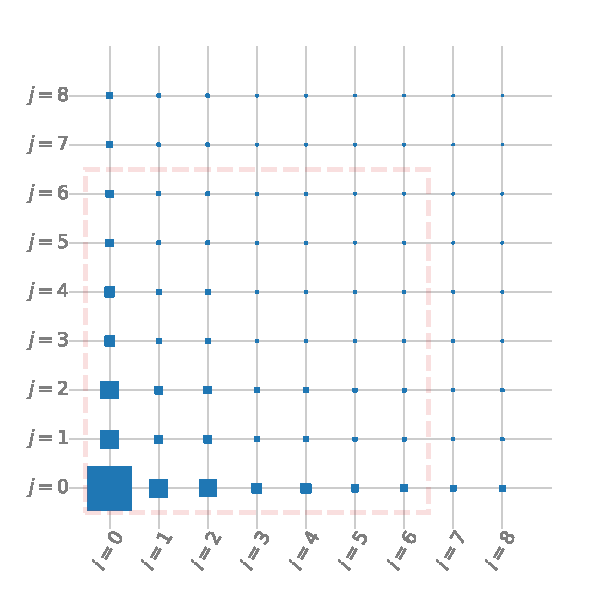
\includegraphics[width=\textwidth]{VFF_decay}
%   \caption{VFF}
%   \label{fig:decay-vff}
% \end{subfigure}\hfil % <-- added
% \begin{subfigure}{0.63\textwidth}
%   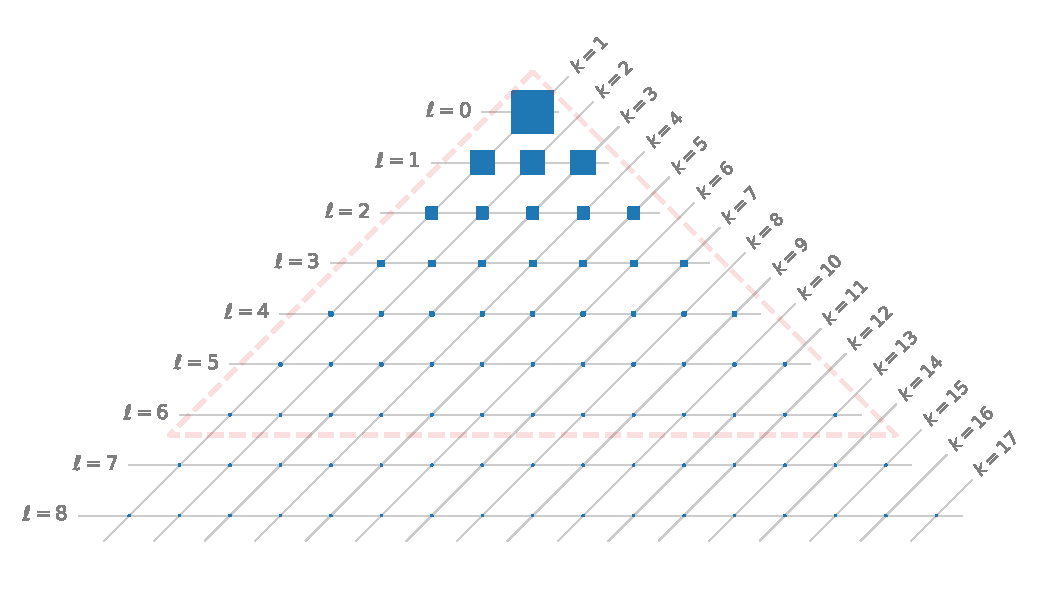
\includegraphics[width=\textwidth]{VISH_decay}
%   \caption{VISH}
%   \label{fig:decay-vish}
% \end{subfigure}\hfil % <-- added
% \caption{Decay rate}
% \label{fig:decay-vff-vs-vish}
% \end{figure}


% The main flaw of VFF comes from the way it generalises to multidimensional input spaces. The approach in~\citet{hensman2017variational} for getting a set of $d$-dimensional inducing functions consists of taking the outer product of $d$ univariate basis and to consider separable kernels so that the elements of $\Kuu$ are given by the product of the inner products in each dimension. For example, in dimension 2, a set of $M^2$ inducing functions is given by $\{(x_1, x_2) \mapsto \psi_i(x_1)\psi_j(x_2)\}_{0 \leq i, j \leq M-1}$, and entries on $\Kuu$ are $\langle \psi_i\psi_j, \psi_k\psi_l \rangle_{\mathcal{H}_{k_1 k_2}^{}}^{} = \langle \psi_i, \psi_k \rangle_{\mathcal{H}_{k_1}^{}}^{} \langle \psi_j, \psi_l \rangle_{\mathcal{H}_{k_2}^{}}^{}$. This construction scales poorly with the dimension: for example choosing a univariate basis as simple as $\{1, \cos, \sin\}$ for an eight-dimensional problem already results in more that 6,500 inducing functions. Additionally, this construction is very inefficient in terms of captured variance, as we illustrate in  \Cref{fig:variance_decay_VFF} for a 2D input space. The figure shows that the prior variance associated with the inducing function $\psi_i(x_1)\psi_j(x_2)$ vanishes quickly when both $i$ and $j$ increase. This means that most of the inducing functions on which the variational posterior is built are irrelevant, whereas some important ones such as $\psi_i(x_1)\psi_0(x_2)$ or $\psi_0(x_1)\psi_j(x_2)$ for $i, j \geq \sqrt{M}$ are important but ignored. Although we used a 2D example to illustrate this poor behaviour, it is important to bear in mind that the issue gets exacerbated for higher dimensional input spaces. As detailed in \cref{fig:variance_decay_SH} and discussed later, our proposed approach does not suffer from such behaviour.

% As is usual in sparse GP methods, the number of inducing variables $M$ is constrained by the computational budget available to the user. Given that we ordered the spherical harmonic by increasing $\ell$, choosing the first $M$ elements means we will select first features with low angular frequency. Provided that the kernel spectral density is a decreasing function (this will be true for classic covariances, but not for quasi-periodic ones), this means that the selected features correspond to the ones carrying the most signal according to the prior. In other words, the decomposition of the kernel can be compared to an infinite dimensional principal component analysis, and our choice of the inducing function is optimal since we pick the ones with the largest variance. This is illustrated in \cref{fig:variance_decay_SH}, which shows the analogue of \cref{fig:variance_decay_VFF} for spherical harmonic inducing functions.

\subsection{Toy Experiment: Banana Classification}

The banana dataset is a 2D binary classification problem \citep{hensman2015scalable}. In \cref{fig:banana} we show three different fits of VISH with $M\in \{9,\ 225,\ 784\}$ spherical harmonics, which correspond respectively to maximum levels of $2$, $14$, and $27$ for our inducing functions. Since the variational framework provides a guarantee that more inducing variables must be monotonically better \citep{titsias2009}, we expect that increasing the number of inducing functions will provide improved approximations. This is indeed the case as we show in the rightmost panel: with increasing $M$ the ELBO converges and the fit becomes tighter.

% While this is expected behaviour for SVGP methods, it is not guaranteed by VFF. Given the Kronecker-structure used by VFF for this 2D experiment \citet{hensman2017variational} report that using a full rank covariance matrix for the variational distribution was intolerably slow. They also show that enforcing the Kronecker structure on the posterior results in an ELBO that {\em decreased} as frequencies were added, and they finally propose a sum-of-two-Kroneckers structure, but provide no guarantee that this would converge to the exact posterior in the limit of larger $M$. In VISH we do not need to impose any structure on the approximate covariance matrix $\MS$, so we retain the guarantee that adding more basis functions will move us closer to the posterior process. The method remains fast despite optimising over full covariance matrices: fitting the models displayed in \cref{fig:banana} only takes a few seconds on a standard desktop.

\begin{figure}[tbh]
    \centering
    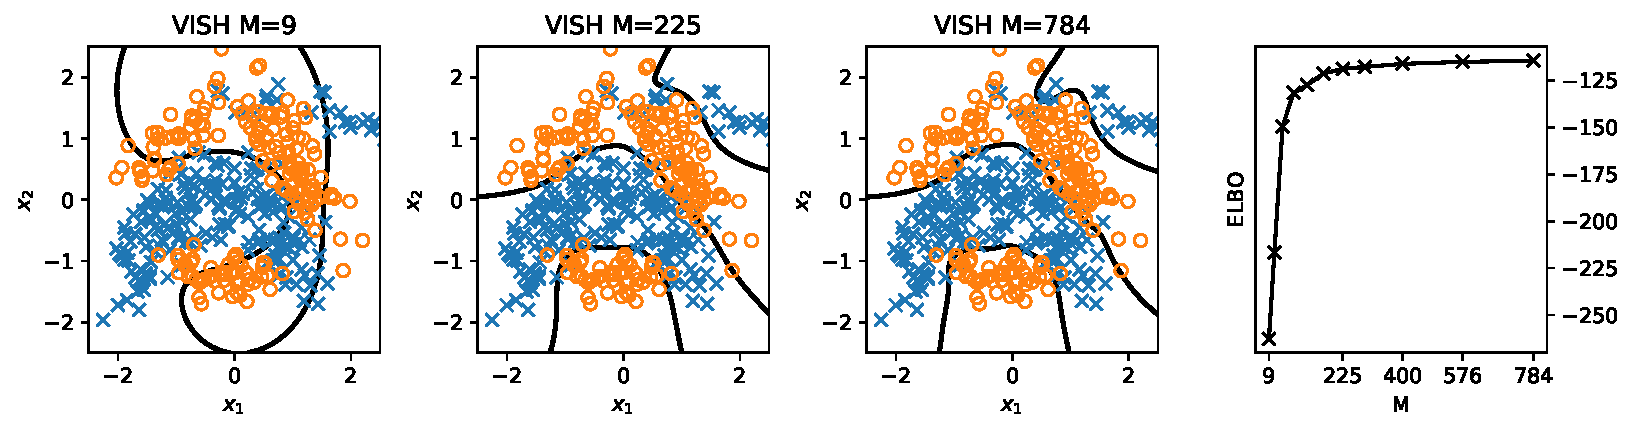
\includegraphics[width=\textwidth]{banana}
    \caption{Classification of the 2D banana dataset with growing number of spherical harmonic basis functions. The right plot shows the convergence of the ELBO with respect to increasing numbers of basis functions.\label{fig:banana}}
\end{figure}



\subsection{Large-Scale Regression on Airline Delay}
 
\begin{table}[tb]
\centering
\resizebox{\textwidth}{!}{\begin{tabular}{lccccccccccc}
    \toprule
    & & \multicolumn{3}{c}{$N=10,000$} & \multicolumn{2}{c}{$N=100,000$} &
    \multicolumn{2}{c}{$N = 1,000,000$}  & 
    \multicolumn{3}{c}{$N = 5,929,413$}        \\
    \cmidrule(lr){3-5}
    \cmidrule(lr){6-7} 
    \cmidrule(lr){8-9} 
    \cmidrule(lr){10-12} 
    Method & M 
    & MSE & NLPD & Time
    & MSE & NLPD
    & MSE & NLPD
    & MSE & NLPD & Time \\
    \midrule
    VISH & 210 & 
    $0.91 \pm 0.16$ &
    $1.328 \pm 0.09$ &
    $1.86 \pm 0.38$ &
    $0.826 \pm 0.052$ &
    $1.28 \pm 0.03$ &
    $0.84 \pm 0.01$ &
    $1.29 \pm 0.01$ &
    $0.833 \pm 0.004$ &
    $1.29 \pm 0.002$ &
    $41.32 \pm 0.81$ \\
    VISH & 660 & 
    $0.90 \pm 0.16$ &
    \bm{$1.326 \pm 0.09$} &
    $4.76 \pm 1.25$ &
    $0.808 \pm 0.052$ &
    \bm{$1.27 \pm 0.03$} &
    $0.83 \pm 0.03$ &
    \bm{$1.28 \pm 0.01$} &
    $0.834 \pm 0.055$ &
    \bm{$1.27 \pm 0.002$} &
    $160.8 \pm 3.80$ \\
    A-VFF & 30\small{/dim.} & 
     \bm{$0.89 \pm 0.15$} &
     $1.362 \pm 0.09$ &
     $6.78 \pm 0.85$ &
     $0.819 \pm 0.05$ &
     $1.32 \pm 0.03$ &
     $0.83 \pm 0.01$ &
     $1.33 \pm 0.03$ &
     $0.827 \pm 0.004$ &
     $1.32 \pm 0.007$ &
     $75.61 \pm 0.75$ \\
    SVGP & 500 & 
     $0.90 \pm 0.16$ &
     $1.358 \pm 0.09$ &
     $836.54 \pm 0.78$ &
     \bm{$0.808 \pm 0.05$} &
     $1.31 \pm 0.03$ &
     \bm{$0.82 \pm 0.01$} &
     $1.32 \pm 0.002$ &
     \bm{$0.814 \pm 0.004$} &
     $1.31 \pm 0.002$ &
     $918.77 \pm 1.21$\\
    \bottomrule
    \end{tabular}
 }
\caption{Predictive mean squared errors (MSEs), negative log predictive densities (NLPDs) and wall-clock time in seconds with one standard deviation based on 10 random splits on the airline arrival delays experiment. Total dataset size is given by $N$ and in each split we randomly select 2/3 and 1/3 for training and testing.}
\label{tab:airline}
\end{table}


This experiment illustrates three core capabilities of VISH: 1) it can deal with large datasets and 2) it is computationally and time efficient 3) the model improves performance in terms of NLPD.

We use the 2008 U.S. airline delay dataset to asses these capabilities. The goal of this problem is to predict the amount of delay $y$ given eight characteristics $x$ of a flight, such as the age of the aircraft (number of years since deployment), route distance, airtime, etc. We follow the exact same experiment setup as \citet{hensman2017variational}\footnote{\url{https://github.com/jameshensman/VFF}} and evaluate the performance on 4 datasets of size 10,000, 100,000, 1,000,000, and 5,929,413 (complete dataset), created by subsampling the original one. For each dataset we use two thirds of the data for training and one third for testing. Every split is repeated 10 times and we report the mean and one standard deviation of the MSE and NLPD. For every run the outputs are normalized to be a centered unit Gaussian and the inputs are scaled to be within $[-1, 1]$.
%for VFF and SVGP. For VISH we normalize the inputs so that each column falls within $[-v_d, v_d]$. The hyperparameter $v_d$ corresponds to the prior variance of the weights of an infinite-width fully-connected neural net layer (see \citet{cho2009kernel}). We can optimise for this weight-variance by back-propagation through $k_u(x)$ w.r.t. the ELBO. This is similar to the lengthscale hyperparameters of stationary kernels.

\Cref{tab:airline} shows the outcome of the experiment. The results for VFF and SVGP are from \citet{hensman2017variational}. We observe that VISH improves on the other methods in terms of NLPD and is within error bars in terms of MSE. Given the variability in the data the GP models improve when more data is available during training.

Given the dimensionality of the dataset, a full-VFF model is completely infeasible. As an example, using just four frequencies per dimension would already lead to $M = 4^8 = 65,536$ inducing variables. So VFF has to resort to an additive model with a prior covariance structure given as a sum of Mat\'ern-3/2 kernels for each input dimension, as in \cref{eq:vff-additive}. Each of the functions $f_d$ is approximated using 30 frequencies.
We report two variants of VISH: one using all spherical harmonics up to degree 3 ($M$=210) and another up to degree 4 ($M$=660). As expected, the more inducing variables, the better the fit.

We also report the wall clock time for the experiments (training and evaluation) for $N=10,000$ and $N=5,929,413$. All these experiments were ran on a single consumer-grade GPU (Nvidia GTX 1070). On the complete dataset of almost 6 million records, VISH took $41\pm0.81$ seconds on average. A-VFF required $75.61\pm0.75$ seconds and the SVGP method needed approximately 15 minutes to fit and predict. This shows that VISH is roughly two orders of magnitude faster than SVGP. A-VFF comes close to VISH but has to impose additive structure to keep its computational advantage.


\section{Conclusion}

We showed, 


In the next chapter, 
